\documentclass[conference]{IEEEtran}
%DIF LATEXDIFF DIFFERENCE FILE
%DIF DEL /home/resort/Documents/repos/DSpaCES2026/regional-energy-twin/manuscript-revised/internal/prose_old.tex   Tue Nov 10 18:18:35 2026
%DIF ADD /home/resort/Documents/repos/DSpaCES2026/regional-energy-twin/manuscript-revised/internal/prose_new.tex   Tue Nov 10 18:18:35 2026
\usepackage{amsmath,amssymb,amsthm}
\usepackage{graphicx}
\usepackage{booktabs}
\usepackage{array}
\usepackage{cite}
\usepackage{balance}
\usepackage[hidelinks]{hyperref}
%DIF 9c9
%DIF < \hypersetup{pdftitle={From Detail to Decisions in Regional Energy Twins},pdfauthor={Alexander V. Mantzaris},pdfsubject={DSpaCES 2026 author-review case-study manuscript}}
%DIF -------
\hypersetup{pdftitle={From Detail to Decisions in Regional Energy Twins},pdfauthor={Alexander V. Mantzaris and James H. Korris},pdfsubject={DSpaCES 2026 camera-ready revision for author review}} %DIF > 
%DIF -------
\newtheorem{proposition}{Proposition}
\newcommand{\R}{\mathbb{R}}
\newcommand{\MarginChecks}{4608}
\newcommand{\MarginCertified}{4608}
\newcommand{\FineGainPercent}{18.3}

\title{From Detail to Decisions in Regional Energy Twins}
\author{\IEEEauthorblockN{Alexander V. Mantzaris}
\DIFdelbegin %DIFDELCMD < \IEEEauthorblockA{School of Data, Mathematical and Statistical Sciences\\
%DIFDELCMD < University of Central Florida\\
%DIFDELCMD < alexander.mantzaris@ucf.edu}%%%
\DIFdelend \DIFaddbegin \IEEEauthorblockA{School of Data, Mathematical\\
and Statistical Sciences\\
University of Central Florida\\
alexander.mantzaris@ucf.edu}
\and
\IEEEauthorblockN{\textcolor{blue}{James H. Korris}}
\IEEEauthorblockA{\textcolor{blue}{Creative Technologies Inc.}\\
\textcolor{blue}{Hollywood, CA, USA}\\
\textcolor{blue}{james.korris@cretecinc.com}}\DIFaddend }
%DIF PREAMBLE EXTENSION ADDED BY LATEXDIFF
%DIF UNDERLINE PREAMBLE %DIF PREAMBLE
\RequirePackage[normalem]{ulem} %DIF PREAMBLE
\RequirePackage{color}\definecolor{RED}{rgb}{1,0,0}\definecolor{BLUE}{rgb}{0,0,1} %DIF PREAMBLE
\providecommand{\DIFaddtex}[1]{{\protect\color{blue}\uwave{#1}}} %DIF PREAMBLE
\providecommand{\DIFdeltex}[1]{{\protect\color{red}\sout{#1}}}                      %DIF PREAMBLE
%DIF SAFE PREAMBLE %DIF PREAMBLE
\providecommand{\DIFaddbegin}{} %DIF PREAMBLE
\providecommand{\DIFaddend}{} %DIF PREAMBLE
\providecommand{\DIFdelbegin}{} %DIF PREAMBLE
\providecommand{\DIFdelend}{} %DIF PREAMBLE
\providecommand{\DIFmodbegin}{} %DIF PREAMBLE
\providecommand{\DIFmodend}{} %DIF PREAMBLE
%DIF FLOATSAFE PREAMBLE %DIF PREAMBLE
\providecommand{\DIFaddFL}[1]{\DIFadd{#1}} %DIF PREAMBLE
\providecommand{\DIFdelFL}[1]{\DIFdel{#1}} %DIF PREAMBLE
\providecommand{\DIFaddbeginFL}{} %DIF PREAMBLE
\providecommand{\DIFaddendFL}{} %DIF PREAMBLE
\providecommand{\DIFdelbeginFL}{} %DIF PREAMBLE
\providecommand{\DIFdelendFL}{} %DIF PREAMBLE
%DIF HYPERREF PREAMBLE %DIF PREAMBLE
\providecommand{\DIFadd}[1]{\texorpdfstring{\DIFaddtex{#1}}{#1}} %DIF PREAMBLE
\providecommand{\DIFdel}[1]{\texorpdfstring{\DIFdeltex{#1}}{}} %DIF PREAMBLE
%DIF LISTINGS PREAMBLE %DIF PREAMBLE
\RequirePackage{listings} %DIF PREAMBLE
\RequirePackage{color} %DIF PREAMBLE
\lstdefinelanguage{DIFcode}{ %DIF PREAMBLE
%DIF DIFCODE_UNDERLINE %DIF PREAMBLE
  moredelim=[il][\color{red}\sout]{\%DIF\ <\ }, %DIF PREAMBLE
  moredelim=[il][\color{blue}\uwave]{\%DIF\ >\ } %DIF PREAMBLE
} %DIF PREAMBLE
\lstdefinestyle{DIFverbatimstyle}{ %DIF PREAMBLE
	language=DIFcode, %DIF PREAMBLE
	basicstyle=\ttfamily, %DIF PREAMBLE
	columns=fullflexible, %DIF PREAMBLE
	keepspaces=true %DIF PREAMBLE
} %DIF PREAMBLE
\lstnewenvironment{DIFverbatim}{\lstset{style=DIFverbatimstyle}}{} %DIF PREAMBLE
\lstnewenvironment{DIFverbatim*}{\lstset{style=DIFverbatimstyle,showspaces=true}}{} %DIF PREAMBLE
%DIF END PREAMBLE EXTENSION ADDED BY LATEXDIFF

\begin{document}
\maketitle

\begin{abstract}
Regional energy twins must connect population demand with local household changes while operating through limited access to detailed measurements. We introduce a controlled evaluation methodology that isolates the contributions of state representation, acquired observations and acquisition decisions. By combining matched evidence comparisons, controlled disturbances and execution tracing, the methodology identifies where refinement improves predictions and where information fails to influence action. We apply it to a retrospective London energy twin built from 167.93 million smart meter rows and 4,194 eligible households, using a hierarchical Gaussian model with GPU inference. Refinement and coarsening preserve registered posterior queries, establishing consistent transitions between regional and household views. Streamed fine inference matches the retained state footprint, showing no capacity advantage for refinement. On real demand backgrounds with synthetic disturbances, full fine access reduces local one hour mean absolute error by \FineGainPercent{}\% relative to the tested adaptive policy, with a larger observation budget. Execution traces reveal that scores respond to 93 of 96 demand disturbances while acquisition schedules remain unchanged, identifying the acquisition gate as a decision bottleneck. A targeted correction changes some schedules but reaches no additional affected meters within the detection window and establishes no acquisition advantage. These findings distinguish forecasting value from successful localization and connect observation access with decision timing. The study provides a reproducible methodology and actionable design criteria for evaluating how regional twins turn local detail into useful information and timely decisions.
\end{abstract}
\begin{IEEEkeywords}
regional digital twins, data spaces, selective observation, Gaussian inference, smart-meter data
\end{IEEEkeywords}




\section{Introduction}
Regional energy twins must connect demand across thousands of households with changes that emerge locally. A stable group total can conceal rising consumption in some households and falling consumption in others. Detecting these changes requires decisions about both representation and observation. A provider may routinely release group totals while supplying individual readings only on request. The consumer must therefore decide which local state to retain, which measurements to acquire and when those measurements can still influence a useful decision. \DIFaddbegin \DIFadd{As an illustrative use case, an energy analytics team could receive group summaries, request selected household readings and use an alarm to prioritize investigation of an unusual local demand pattern. Missed localization would leave the team unable to identify which sampled household group to examine. This is a possible use of the interface, not a deployment or measured operational benefit.
}\DIFaddend 

These choices have different consequences. Exposing household predictions from an existing model can leave its information unchanged. Acquiring new readings can update both household and regional predictions through their shared uncertainty. Receiving informative observations, however, does not ensure that an acquisition policy acts on them. Scores pass through thresholds, rankings and budget rules, and additional readings must arrive before the relevant decision deadline. Evaluating only forecast error or memory consumption leaves the source of an improvement, or the cause of a failure, unresolved.

We \DIFdelbegin \DIFdel{introduce a controlled evaluation methodology that connects these stages within one regional twin. Its methodological contribution is the integration of }\DIFdelend \DIFaddbegin \DIFadd{connect }\DIFaddend comparisons under identical evidence, controlled tests of aggregate visibility and \DIFdelbegin \DIFdel{detailed tracing from observations to acquisition decisions. This design distinguishes the value of changing representation from the value of receiving more information , then identifies where the acquisition process prevents that information from improving outcomes. It provides a practical basis for assessing whether an apparent refinement benefit justifies additional storage, measurement access or decision complexity}\DIFdelend \DIFaddbegin \DIFadd{execution tracing within one regional twin. This separates representation from information gains and identifies barriers between observations and decisions}\DIFaddend .

We apply the methodology to a retrospective twin of the sampled Greater London household population. Low Carbon London supplies real measurements recorded every half hour~\cite{london}. Simulated providers expose group summaries and requested household readings through an explicit interface. A fixed hierarchical Gaussian model supports regional, group and household queries with GPU inference. Keeping this model fixed enables controlled comparisons of representation, acquired evidence and observation selection.

Three questions organize the study. \textbf{RQ1.} What does changing representation preserve under identical evidence, and what resources does it require? \textbf{RQ2.} What forecasting and detection value do fine observations provide when aggregation hides local disturbances? \textbf{RQ3.} Can the tested acquisition policy obtain useful additional information within its observation budget and detection window?

The study delivers three connected contributions.
\begin{enumerate}
\item \textbf{Attribution of refinement benefits.} Comparisons under identical evidence verify preservation of registered posterior queries through refinement and coarsening. Retained state falls from 61.12 to 21.60 MB, matching streamed fine inference.
\DIFdelbegin \DIFdel{This establishes a concrete control for distinguishing storage savings from increased capacity or improved predictions.
}\DIFdelend \item \textbf{Measurement of local information value.} Controlled disturbances separate aggregate visibility, forecasting and localization. Full fine access improves local forecasts at a larger observation budget, while all methods miss localization of the 16 original exact cancellation events.
\DIFdelbegin \DIFdel{These results show what additional measurements contribute and why forecasting gains alone cannot validate a monitoring capability.
}\DIFdelend \item \textbf{Diagnosis of acquisition barriers.} Execution traces reveal responsive scores in 93 of 96 demand episodes without any acquisition schedule change. A targeted correction exposes late requests and a remaining alarm barrier without establishing an acquisition advantage.
\DIFdelbegin \DIFdel{The diagnosis gives designers specific mechanisms to inspect when informative observations fail to produce timely action.
}\DIFdelend \end{enumerate}

Established Gaussian and observability results support the analysis. \DIFdelbegin \DIFdel{The methodological value lies in connecting these principles to controlled comparisons and observable execution behavior. }\DIFdelend Code, configurations, traces and reproduction scripts are available~\cite{artifact}. \DIFdelbegin \DIFdel{Within this retrospective study, real observations and synthetic disturbances provide a reproducible basis for evaluating how regional twins convert local detail into predictive and operational value}\DIFdelend \DIFaddbegin \DIFadd{The contribution is diagnostic, not a validated operational system: M3 provides virtually no advantage over random acquisition, and M3b does not establish an advantage. The practical checks are to hold evidence fixed, benchmark capacity against streaming, inspect gate margins and acquisition deadlines, compare detection at comparable false-alarm rates, and assess predictive calibration separately from numerical consistency (Table~\ref{tab:guidance})}\DIFaddend .



\section{Related Work and Scope}
Multiresolution inference represents local and global uncertainty through hierarchical bases~\cite{katzfuss2017}. Multiresolution filters propagate covariance approximations, with exactness in identified special cases~\cite{mrf}. Hierarchical sparse Cholesky methods exploit specified conditional structure for scalable filtering~\cite{vecchia}. Our exact conditional calculations in a smaller fixed model isolate representation from observation access.

Distributed low rank inference exchanges local sufficient quantities to recover a centralized posterior~\cite{distributed}, providing the closest mathematical baseline for our shared state and private detail model. Incremental methods such as iSAM2 reuse conditionals within a Bayes tree~\cite{isam}. Because locality depends on separator size, ordering and coupling, our comparisons include conventional message reuse and streamed prediction.

MinT reconciles forecasts with aggregation constraints by minimizing forecast error covariance trace under its assumptions~\cite{mint}. Our regional and local queries come from one joint model, ensuring algebraic agreement while leaving accuracy and calibration to empirical evaluation.

Event triggered estimation distinguishes measurements from information conveyed by transmission decisions. Sun and Work represent nontransmission through synthetic measurements~\cite{sun}. Han et al. develop stochastic triggers that preserve Gaussian estimation under specified assumptions~\cite{han}. Our heuristic uses scheduled probes and omits selection information outside its finite inference window, so those guarantees do not apply.

Controlled sensing jointly selects observations and a stopping rule. Veeravalli et al. establish first order asymptotic optimality under finite action and postchange parameter sets, specified observation laws and a mean time to false alarm criterion~\cite{controlled}. Our fixed reading budget and empirical thresholds address a different setting. Random acquisition provides a simple, nonoptimal comparator.

Electricity anomaly detection can use detailed inputs before producing aggregate decisions. He et al. combine participant features with a localization rule~\cite{he}. Their observation interface differs from a consumer receiving summaries and requesting limited fine readings. We therefore distinguish model dimension from information access.
\DIFdelbegin \DIFdel{Our contribution connects these established methods through a controlled empirical design. Comparisons hold evidence fixed to assess representation, vary access to measure information value and trace acquired signals through decision code. This identifies where consistent probabilistic refinement and observable local changes fail to improve acquisition, providing practical guidance for evaluating observation policies alongside representation choices.
}\DIFdelend 




\section{Regional Twin and Information Interfaces}
\subsection{Physical observations and study population}
Readings measure electricity consumed in half hour intervals, in kWh. Forecasts one and six hours ahead target readings two and 12 intervals later, respectively, rather than cumulative consumption over those horizons. We retain meter identifiers and source clock labels. Verified feeders, borough assignments, coordinates and population expansion weights are unavailable.

The archive contains 167,932,474 rows, 167,817,021 distinct meter/time keys and 5,566 meter identifiers, compared with the catalog's approximate 167 million readings and 5,567 households~\cite{london}.
\DIFdelbegin \DIFdel{The 801.67 MB ZIP expands to 8.54 GB of CSV and yields 528.82 MB of typed, partitioned Parquet. Streaming ingestion processes about 472,000 rows/s with 3.36 GB peak host memory. These figures describe ingestion performance rather than inference throughput.
}\DIFdelend 

Nonfinite, invalid and negative readings become missing values. Duplicate keys are retained deterministically for archival bookkeeping but excluded from fitting and replay. Missing outcomes are never replaced with zero. Unresolved timezone and daylight saving semantics require excluding accessible clock transition days without assuming UTC alignment.

Eligibility uses only 2012 data and requires at least 8,760 valid readings per household. The 4,194 eligible households provide 52,109,356 valid training readings, with 29.3\% of the rectangular grid missing. Standard tariffs cover 3,362 households and time of use tariffs cover 832. These labels are descriptive, without estimating tariff effects. January to March 2013 supplies exploratory development replay. April to December 2013 and outcomes from the earlier building data project remain sealed. Ingestion partitions withheld records, whose values are excluded from fitting, selection and scoring.

\subsection{One fixed probabilistic model}
Let $y_{it}$ denote household $i$'s recorded demand. The model is
\begin{align}
 s_{t+1}&=F_s s_t+\eta_t,\\
 y_{it}&=\mu_{i,\ell(t)}+\ell_i^\top s_t+d_{it}+\epsilon_{it},\label{eq:model}\\
 d_{i,t+1}&=\rho_i d_{it}+\zeta_{it}.
\end{align}
Here $s_t\in\R^{16}$ captures common variation, $\mu_{i,\ell(t)}$ is a weekly seasonal profile with 336 slots, and $d_{it}$ is a private household residual. Loadings, dynamics and noise conventions are fitted on training data. Missing standardized residuals receive mean values only for initial factor construction. Loadings are then refitted on observed entries. Private residual covariance uses a fixed 80\% autoregressive and 20\% nugget split, with persistence clipped to $[-0.95,0.95]$. The common transition has spectral radius 0.9942. These are working Gaussian assumptions.

Private innovations are conditionally independent given the common state. Household forecast errors are not unconditionally independent. Regional variance includes common state uncertainty, future common process noise, private temporal dependence and measurement noise. Gaussian predictions permit negative demand, whereas disturbance generation enforces nonnegative replay observations and targets.

Sixteen groups, formed by sorted physical meter index modulo 16, contain 262 or 263 households each. \DIFdelbegin \DIFdel{They are synthetic populations without geographical assignments}\DIFdelend \DIFaddbegin \DIFadd{These synthetic groups are not verified districts or feeders. Spatially meaningful groups could change shared demand dependence, the extent of cancellation within a released sum and localization difficulty; their effect is unmeasured here}\DIFaddend . The window contains 24 half hour steps\DIFdelbegin \DIFdel{, giving a common separatordimension of }\DIFdelend \DIFaddbegin \DIFadd{. Its common separator, the shared latent trajectory connecting household factors, has dimension }\DIFaddend $16\times24=384$. \DIFdelbegin \DIFdel{All private trajectories together yield }\DIFdelend \DIFaddbegin \DIFadd{Counting every latent component at every window step gives }\DIFaddend 101,040 formal coordinates at the largest cohort, without constructing a dense covariance of that size.
\DIFdelbegin \DIFdel{Source records contribute to fitted statistics without residing simultaneously in GPU memory.
}\DIFdelend 

\begin{figure*}[!t]
\centering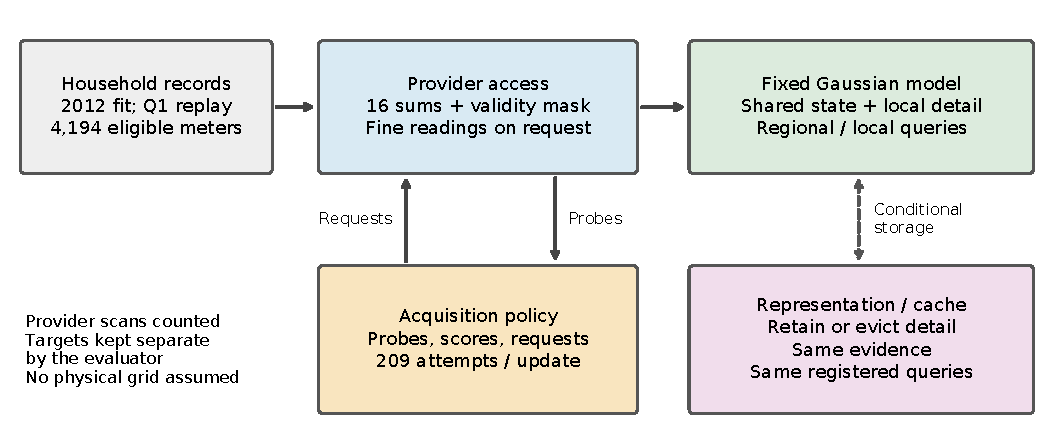
\includegraphics[width=\textwidth]{figures/information_flow.pdf}
\caption{Separating access from representation identifies the value of detail. Providers supply summaries and requested fine readings. Acquired probes guide requests, while representation controls conditional storage without adding evidence. One model answers regional, group and household queries. Provider summary scans are counted separately from consumer fine reads.}
\label{fig:interfaces}
\end{figure*}




\subsection{Provider summaries, fine access and query support}
Each update supplies 16 group sums over observed households and a native missingness mask. Constructing these summaries \DIFdelbegin \DIFdel{requires a charged providerscan}\DIFdelend \DIFaddbegin \DIFadd{reads all household values at the provider; this scan is counted as provider work, separately from consumer access}\DIFaddend . Fine access enforces the current cutoff, unique requests and an observation budget. Unrevealed household residuals cannot guide acquisition.

Restricted methods allow $\lfloor0.05\times4194\rfloor=209$ requests per update, including 41 rotating probes. Missing readings consume attempts without contributing likelihood. A cache retains finite acquisitions for 24 steps. Requests, finite returns and assimilation are logged separately. \DIFaddbegin \DIFadd{Informative exposure additionally requires a finite reading actually altered by the disturbance; requesting an affected identity alone does not establish it. }\DIFaddend Figure~\ref{fig:interfaces} separates these operations and Table~\ref{tab:methods} defines the interfaces. Every method supports conditional household predictions, including those receiving only aggregates.




\begin{table*}[!t]
\caption{Interfaces for shock comparisons. All methods share the fitted model, 16 group sums and missingness masks. Attempts include missing readings. Fine access describes available evidence rather than model dimension.}
\label{tab:methods}\centering
\begin{tabular}{p{.14\textwidth}p{.25\textwidth}p{.26\textwidth}p{.25\textwidth}}
\toprule
Method & Additional observations & Acquisition rule & Comparison role\\
\midrule
M0 Aggregate & None & Aggregate change detector & Conditional household predictions\\
M1 Probes & 41 fixed rotating probes & Same monitoring as M3 & Probe information control\\
M2 Random & 41 probes + 168 random requests & Uniform selection without replacement & Matched observation budget\\
M3 Gated & 41 probes + 168 extra requests & Threshold and hold. 42 explore, up to 126 target one group & Original adaptive policy\\
M3b Ranked & Same 209 attempts & Highest positive score with unchanged exploration & Frozen ranking correction\\
Fixed trace & M3 or M3b trace, delivered sequentially & No future acquisition decisions & Conventional retention under identical evidence\\
M4 Full fine & All 4,194 household records & Streamed full access & Structured full information reference\\
\bottomrule
\end{tabular}
\end{table*}

Regional targets sum valid household readings, using identical support for every method's predictions and uncertainty. These posterior queries measure observed support rather than complete population demand. Future validity masks affect only scoring weights, never the posterior information matrix or acquisition inputs. Monitoring uses a separate prediction one step ahead on full support. Model selection and policies never access future consumption. The unmodified refinement panel has no complete cohort totals, with target support ranging from 4,082 to 4,168 households.








\section{Principles for Consistent Regional Refinement}
\subsection{Preserving queries as detail changes}
Gaussian elimination supports verifiable refinement. \DIFaddbegin \DIFadd{A registered posterior query is a specified forecast quantity whose conditional mean, covariance and mapping are retained for later evaluation. }\DIFaddend Let $c$ denote retained coordinates and $d$ detail coordinates in a proper Gaussian posterior with precision $J$ and information vector $h$. For $J_{dd}\succ0$,
\begin{align}
J_c&=J_{cc}-J_{cd}\operatorname{solve}(J_{dd},J_{dc}),\label{eq:schur}\\
h_c^{\rm marg}&=h_c-J_{cd}\operatorname{solve}(J_{dd},h_d).
\end{align}
The conditional mean of $d$ is $\operatorname{solve}(J_{dd},h_d-J_{dc}c)$ and its covariance is $J_{dd}^{-1}$. Factor solves implement these established identities without explicit inversion~\cite{distributed,isam}.

\begin{proposition}[Registered query preservation]
For a fixed model, evidence and window, suppose
$q\mid c\sim\mathcal N(a+Lc,V)$ and $c\sim\mathcal N(m,C)$. In exact arithmetic, retaining $(a,L,V,m,C)$ preserves the query mean $a+Lm$ and covariance $V+LCL^\top$ when other detail is evicted. Reconstruction with the original conditionals preserves these quantities regardless of elimination order.
\end{proposition}
\begin{proof}
Iterated expectation and total covariance give the stated moments. Integrating a proper Gaussian over a fixed coordinate set produces the same marginal in any order. Combining that marginal with its original conditional recovers the joint distribution.
\end{proof}

\DIFdelbegin \DIFdel{This identifies the information needed for consistent regional and household queries. }\DIFdelend The panel registers full group totals, common observed support totals and one fixed household per group at each lead, including covariances within each lead. New household combinations or joint queries across leads may require reconstruction. Conditional information is essential. Both $d=c+e$ and $d=-c+e$, with independent $c,e\sim\mathcal N(0,1)$, share the same coarse marginal but have opposite cross covariances. Resource accounting includes conditionals and host caches.

Evidence integration preserves consistency when acquired readings contribute to an existing group sum. The update uses
\begin{equation}
p(y_{\rm fine},a\mid c)
=p(y_{\rm fine}\mid c)\,p(a\mid y_{\rm fine},c),\label{eq:replace}
\end{equation}
conditioning the sum on acquired values and native masks. All constituents together make the remaining aggregate likelihood redundant. Versioned evidence replaces the old group message atomically, preventing duplicate evidence. A duplicate evidence control confirms the posterior changes.

Conditionally private groups permit reuse of unaffected messages within a window, followed by refactorization of the common separator. Update cost depends on block size and coupling. With rank $r=16$, window length $L=24$ and $N$ households, storage is $O(NL^2)$ for private temporal covariance plus separator and query summaries. Dense separator factorization costs $O((rL)^3)$, while private temporal factors support GPU batching. This locality depends on conditional structure and can diminish with stronger coupling or factorization fill. Each advancing window restarts from the fixed training prior and rebuilds all 16 group factors \DIFdelbegin \DIFdel{, without propagating an exact boundary messagefrom the complete history}\DIFdelend \DIFaddbegin \DIFadd{without passing a boundary message. This discards observation information before the window and can affect forecasts and uncertainty; the size and direction of that effect were not evaluated}\DIFaddend .







\subsection{Aggregate visibility and information value}
For household perturbation $d_t$ and summary operator $S_t$, the observable change is $S_t d_t$. Our hidden controls cancel within every observed group, accounting for missing readings. This tests visibility through the actual provider interface, including group totals.

For a fixed linear state model with household demand $Hx_t$, transition $F$ and macro mapping $C=SH$, the standard observability matrix~\cite{hespanha} is
\begin{equation}
\mathcal O_L=\begin{bmatrix}C^\top&(CF)^\top&\cdots&(CF^L)^\top\end{bmatrix}^{\!\top}.
\end{equation}
\begin{proposition}[Indistinguishability over a finite horizon]
Consider two linear systems whose initial states differ by deterministic $\delta$, with identical dynamics, inputs and joint noise laws. If $\mathcal O_L\delta=0$, their macro observation distributions coincide through time $L$. Any detector using only these observations and the same independent randomization has equal alarm probability under both systems.
\end{proposition}
\begin{proof}
Couple the systems with identical noise draws. Their state difference at time $k$ is $F^k\delta$, giving macro observation difference $CF^k\delta=0$. The observation laws therefore coincide, as do the output laws of any detector using them.
\end{proof}

\DIFdelbegin \DIFdel{This criterion gives the study a principled way to distinguish unavailable information from unsuccessful detection. }\DIFdelend Additional probes can reveal hidden directions when their observation operators respond to those changes. Detection performance then depends on signal strength, noise and the decision rule.

As an algebraic illustration, changes of $+1$ and $-1$ kWh within one group cancel immediately. Illustrative persistence factors of 0.96 and 0.70 produce a later sum of $0.96^k-0.70^k$, reaching 0.26 kWh after one step and 0.4316 after two. Equal persistence preserves cancellation. This distinguishes changes requiring local observations from those becoming visible through later aggregates. Replay disturbances overlay measured demand rather than follow this illustrative generator, so their visibility is verified directly through $S_t d_t$.







\subsection{Tracing information into acquisition decisions}
\DIFdelbegin \DIFdel{We connect observation sensitivity with decision behavior by pairing the acquisition policy with a verifiable test of gate stability. This identifies where informative measurements influence requests and where the decision mechanism blocks their effect.
}%DIFDELCMD < 

%DIFDELCMD < %%%
\DIFdelend M3 first requests its 41 probes. \DIFaddbegin \DIFadd{An acquired fine innovation is the difference between an actually returned household reading and its predicted value. }\DIFaddend For each finite probe reading, \DIFdelbegin \DIFdel{it }\DIFdelend \DIFaddbegin \DIFadd{M3 }\DIFaddend computes $z_{it}=|y_{it}-\widehat y^{\rm coarse}_{it}|/\sqrt{v^{\rm coarse}_{it}}$. The reference is the previous forecast one step ahead using aggregates alone, initialized from the training seasonal profile. Group scores follow
\begin{equation}
q_{gt}=0.8q_{g,t-1}+\max\{0,\max_{i\in P_t\cap g}z_{it}-2\},\label{eq:score}
\end{equation}
where an empty probe group contributes zero. If $\max_gq_{gt}>\tau$, with $\tau=13.4334$, M3 selects the group with the highest score and resets a hold lasting four decisions. Otherwise it retains a held group or becomes inactive. Of 168 additional attempts, 42 explore and up to 126 target the active group. All additional attempts rotate when inactive. Probe values can influence current requests. Additional readings update inference but never enter acquisition scores. \DIFaddbegin \DIFadd{The decay 0.8 and offset 2 are fixed heuristics in both the configuration and executable policy, not fitted or sensitivity-tuned parameters. The threshold is the 98th percentile of the probe-only M1 maximum scores on the 88 post-startup calibration updates described below, yielding 13.4333767. The gate diagnosis is conditional on these settings.
}\DIFaddend 

\begin{proposition}[Sufficient condition for acquisition gate stability]
Let $b=\max_gq_g$, $b'=\max_gq'_g$, and $e=\|q'-q\|_\infty$. If $e<|b-\tau|$, the strict decisions $b>\tau$ and $b'>\tau$ coincide. Equality or a zero margin leaves this condition inconclusive.
\end{proposition}
\begin{proof}
The maximum is Lipschitz with constant one in the infinity norm, giving $|b'-b|\le e$. The strict margin condition prevents the perturbed maximum from reaching or crossing the threshold.
\end{proof}

\DIFdelbegin \DIFdel{This elementary bound turns score changes into a checkable explanation of threshold behavior. }\DIFdelend We complete the diagnosis by auditing ordered meter and time requests and finite assimilation, accounting for ranking, ties, hold state, remaining budget and available identities.
\DIFdelbegin \DIFdel{Pairing the margin test with actual execution traces distinguishes responsive scores from changed acquisitions. The resulting analysis gives twin designers a reproducible way to locate decision barriers before investing in additional observations or more detailed representations.
}\DIFdelend 









\section{Experimental Protocol}
\subsection{Complementary evaluation cohorts}
Three complementary panels connect representation consistency, disturbance response and acquisition behavior. \textbf{A, the unmodified refinement panel,} evaluates 32 development origins across four weeks with nested populations of 1,024, 2,048 and 4,194 households. Fixed, random and uncertainty guided schedules open 2, 4 or 8 groups, yielding 864 policy cases and 1,728 restoration cycles. These controlled computational comparisons share backgrounds and are not independent physical episodes.

\textbf{B, the original disturbance panel,} tests information value through 112 sequential episodes on eight backgrounds from those four weeks. Crossing six disturbance families with two magnitudes produces 96 demand episodes. Eight unmodified and eight measurement fault episodes provide controls. Each episode includes 23 summary initialization intervals, 48 scored updates and targets through six hours ahead.
\DIFdelbegin \DIFdel{Freezing locations, seeds and amplitudes before scoring supports reproducible comparisons.
}\DIFdelend 

\textbf{C, the corrective panel,} tests the diagnosed acquisition mechanism on four predetermined midday backgrounds reused from B. Localized, exactly cancelling, delayed aggregate and unmodified conditions produce 12 demand episodes with fresh seeds and four controls. The panel uses the higher nominal magnitude, with seed parity producing localized increases. Its scope excludes localized decreases and other onset contexts. Four original episodes support diagnosis separately from C. Reconstructing B's 112 episodes verifies execution without adding independent evidence.
\DIFdelbegin \DIFdel{Keeping panel comparisons separate preserves the interpretation of corrective results and avoids treating differences between B and C as temporal model deterioration.
}\DIFdelend 




\subsection{Controlled disturbances and calibrated comparisons}
Reversible overlays produce $y^{\rm shock}_t=y^{\rm background}_t+d_t$, with the same perturbed series supplying observations and future demand targets. Broad increases test macro detection, while localized increases and decreases test sensitivity to small subsets. Opposing changes create exact or approximate cancellation within groups. Different persistence introduces delayed aggregate effects, and ramps test gradual change. Sensor fault controls alter readings alone, separating measurement errors from demand changes.

Magnitudes follow training residual scales. Decreases are capped at 80\% of available demand, and paired changes are suppressed where missing support is incompatible. Realized amplitudes can therefore differ from nominal scales. Cancellation is verified after these operations, retaining null and attenuated realizations. These controls test information access on real trajectories using synthetic disturbances, without modeling grid topology or physical fault propagation.

The unmodified January \DIFdelbegin \DIFdel{3 to 4 }\DIFdelend \DIFaddbegin \DIFadd{3--4, 2013 }\DIFaddend segment supplies 96 \DIFaddbegin \DIFadd{half-hour }\DIFaddend calibration updates. Excluding \DIFdelbegin \DIFdel{eight startup updates , empirical quantiles set }\DIFdelend \DIFaddbegin \DIFadd{steps 0--7 leaves 88 updates for }\DIFaddend acquisition and alarm \DIFdelbegin \DIFdel{thresholds }\DIFdelend \DIFaddbegin \DIFadd{threshold quantiles, }\DIFaddend without injected event labels. Alarms use the maximum \DIFdelbegin \DIFdel{across group and legally acquired fine }\DIFdelend \DIFaddbegin \DIFadd{of normalized group and acquired household }\DIFaddend innovations at each update, targeting 2\%. Each method is calibrated for the number and distribution of its exposed readings. This separates the alarm criterion from M3's acquisition gate.

M3b isolates that gate's role by retaining Eq.~\eqref{eq:score}, probes, model, budget and exploration while assigning the extra budget to the current highest positive score. Its alarm is calibrated separately on the same segment. The correction was fixed before comparison, without searching policy variants. Conventional retention references receive M3 or M3b's trace sequentially, without future requests. M4 uses structured streamed inference with all available readings. Panel A's uncertainty policy remains a diagnostic without further tuning.

Intervals include future process and measurement uncertainty. Raw central 90\% intervals use 1.6449 standard deviations. Adjusted \DIFdelbegin \DIFdel{intervals use empirical absolute standardized error quantiles from }\DIFdelend \DIFaddbegin \DIFadd{prediction intervals use absolute standardized-error quantiles over all 96 calibration forecast origins, separately from the 88-update alarm }\DIFaddend calibration. Coverage remains empirical because of serial dependence, model misspecification and adaptive selection. Historical acquisition decisions can depend on observations outside the retained window, whose selection effects are not modeled. Agreement under identical evidence therefore verifies computational consistency of the working posterior, with historical selection effects outside its scope.

\subsection{Outcome measures and paired evaluation}
\DIFdelbegin \DIFdel{Detection requires an alarm at lags 0 through 6 }\DIFdelend \DIFaddbegin \DIFadd{Panel B's original scoring code uses lags 0--5 }\DIFaddend after onset, \DIFdelbegin \DIFdel{covering seven observation instants over }\DIFdelend \DIFaddbegin \DIFadd{six instants within a three-hour interval; panel C uses lags 0--6. Table~\ref{tab:results} preserves both original counts. The earlier uniform description as lags 0--6 was incorrect for B. The new alarm-threshold comparison explicitly uses lags 0--6 inclusive, seven instants through }\DIFaddend three hours. \DIFdelbegin \DIFdel{Correct }\DIFdelend \DIFaddbegin \DIFadd{Original correct }\DIFaddend localization requires an alarmed group that is currently affected within \DIFdelbegin \DIFdel{that }\DIFdelend \DIFaddbegin \DIFadd{the respective panel's }\DIFaddend window. Misses receive a delay of seven half hour steps, retaining failures in delay averages. A hit does not relabel all event times as successes. Control alarm rates divide alarmed updates by all unmodified updates, with false household and group localizations recorded separately.

Local mean absolute error (MAE) averages valid affected household errors within target intervals, then event intervals and episodes. Panel B uses 80 episodes from five local families, excluding broad shifts and controls. Panel C uses 12 demand episodes. Forecasts are evaluated by target time, including targets predicted before a disturbance was observable. Regional comparisons exclude exactly cancelling events, whose unchanged regional MAE cannot indicate refinement value.

Pairing identical backgrounds, overlays and target support isolates differences between methods. All background differences are displayed after averaging families and magnitudes within each background. The eight backgrounds span four weeks, with C reusing one per week. Results are descriptive, without assuming independent households or hours, claiming significance or treating similar averages as equivalence. \DIFdelbegin \DIFdel{Reporting realized alarm rates alongside the frozen operating point connects performance to deployment behavior. }\DIFdelend Only executed sequential policy comparisons support claims of acquisition improvement.




\subsection{GPU implementation and resource accounting}
Fitting and replay use double precision (FP64) on an NVIDIA RTX PRO 4500 Blackwell with 32,623 MiB of reported memory. The CPU handles ingestion, provenance, coordination and analysis. Inference batches household temporal factors and solves a common separator system. Linear solves produce means and aggregate covariances, including uncertainty from shared future noise.

Resource accounting separates provider scans, consumer requests, payload sizes, transfers, retained state and total update time. Payload estimates describe simulated communication rather than measured network traffic or Parquet storage. Scoring data do not supply the estimator with additional readings. Total update costs include setup and cache restoration. Earlier shared matrix solver tests found no acceleration advantage, and we claim no CPU versus GPU speedup.









\section{Results}
\subsection{RQ1. Query consistency and information transfer}
The regional twin supports changes in retained detail while preserving registered predictions across all 864 cases. Query means and variances remain consistent through refinement and eviction. Policy round trips show zero recorded discrepancy. Broader restoration checks, including streamed fine reconstruction, reach $1.42\times10^{-14}$, while incremental and rebuilt separator means differ by at most $4.14\times10^{-15}$. These FP64 results demonstrate reliable numerical transitions between representations within the tested model.
\DIFdelbegin \DIFdel{Forecast accuracy provides a separate measure of predictive value.
}\DIFdelend 

At 4,194 households and eight active groups, eviction reduces retained state from 61.12 MB to 21.60 MB. Streamed fine inference achieves the same footprint. \DIFdelbegin \DIFdel{The comparison identifies a practical storage and restoration tradeoff while establishing conventional streaming as the relevant capacity baseline. }\DIFdelend Initial summaries, private covariance storage, host caches and reconstruction costs remain part of the implementation.
\DIFdelbegin \DIFdel{The demonstrated capability is consistent control of retained detail, with no additional capacity advantage over streaming.
}\DIFdelend 

A concrete example demonstrates how new evidence connects regional and household predictions. At the first replay origin, exposing detail preserves the regional mean of 988.287 kWh and a selected household mean of 0.5630 kWh. Acquiring readings from eight groups updates these predictions to 984.012 and 0.6666 kWh. Through the shared state, a selected household in an unopened group also changes from 0.5012 to 0.6057 kWh. The twin therefore distributes information across scales without acquiring fine readings from every group. These values are model predictions rather than observed population totals or causal demand effects.
\DIFdelbegin \DIFdel{For consumers, this demonstrates the distinct roles of accessing existing conditional predictions and acquiring evidence that updates them.
}\DIFdelend 

The largest cohort also reveals an acquisition design constraint. Its uncertainty guided schedule remains static because Gaussian conditional variance scores do not depend on newly observed values. With eight groups, regional MAE one hour ahead is 39.082 kWh versus 37.599 for random selection, a 3.94\% disadvantage. Nominal 90\% intervals cover 59.4\% of the 32 scored origins.
\DIFdelbegin \DIFdel{This comparison identifies observation sensitivity and calibration as concrete priorities for acquisition design under the tested model and budget.
}\DIFdelend 








\begin{table*}[!t]
\caption{Fine observations improve forecasts without establishing an acquisition advantage. Results use recorded episode artifacts. B is the original disturbance panel and C the corrective panel. Local MAE one hour ahead is in kWh per affected household, using 80 local episodes in B and 12 in C. \DIFdelbeginFL \DIFdelFL{Detection }\DIFdelendFL \DIFaddbeginFL \DIFaddFL{Original detection }\DIFaddendFL and correct group localization use \DIFdelbeginFL \DIFdelFL{all }\DIFdelendFL \DIFaddbeginFL \DIFaddFL{lags 0--5 for B's }\DIFaddendFL 96 \DIFdelbeginFL \DIFdelFL{and 12 }\DIFdelendFL demand episodes \DIFdelbeginFL \DIFdelFL{, respectively. }\DIFdelendFL \DIFaddbeginFL \DIFaddFL{and lags 0--6 for C's 12. }\DIFaddendFL Control alarms use unmodified episodes. Delay includes misses at 3.5 h. Representations receiving identical evidence match their source policy and are omitted as duplicate rows.}
\label{tab:results}\centering
\begin{tabular}{lrrrrr}\toprule
Method & Local MAE & Detected & Localized & Alarmed control updates & Mean delay (h)\\\midrule
\multicolumn{6}{l}{\textit{B: original disturbances}} \\
M0 Aggregate & 0.1777 & 37/96 & 20/96 & 36/384 & 2.44 \\
M1 Probes & 0.1762 & 17/96 & 11/96 & 15/384 & 3.03 \\
M2 Random & 0.1710 & 33/96 & 14/96 & 25/384 & 2.64 \\
M3 Gated & 0.1696 & 29/96 & 15/96 & 30/384 & 2.66 \\
M4 Full fine & 0.1386 & 42/96 & 15/96 & 41/384 & 2.24 \\
\multicolumn{6}{l}{\textit{C: corrective check}} \\
M0 Aggregate & 0.2752 & 10/12 & 5/12 & 19/192 & 1.38 \\
M2 Random & 0.2667 & 8/12 & 2/12 & 14/192 & 2.17 \\
M3 Gated & 0.2621 & 6/12 & 2/12 & 15/192 & 2.29 \\
M3b Ranked & 0.2660 & 4/12 & 2/12 & 14/192 & 2.71 \\
M4 Full fine & 0.2053 & 9/12 & 3/12 & 31/192 & 1.33 \\
\bottomrule\end{tabular}

\end{table*}

\subsection{RQ2. Quantifying the value and cost of fine observations}
Fine observations provide a measurable improvement in local forecasting. In the original disturbance panel B, full fine inference reduces local MAE one hour ahead from gated M3's 0.1696 to 0.1386 kWh, a \FineGainPercent{}\% reduction obtained with a larger observation budget. Comparisons under identical evidence attribute this improvement to acquired data. At the restricted budget, M3's average advantage over random acquisition is 0.00145 kWh or 0.85\%. Table~\ref{tab:results} reports B and the corrective panel C separately, while Figure~\ref{fig:paired} displays paired background differences.
\DIFdelbegin \DIFdel{These controls separate additional data access from acquisition policy effects.
}\DIFdelend 

Disturbance families test each observation interface. Every method detects broad increases of nominal magnitude three on all eight backgrounds, demonstrating effective macro detection of widespread changes. All methods, including random and streamed fine inference, correctly localize zero of B's 16 exact cancellation events within the detection window. For these events, aggregation removes the macro signature and available fine readings do not trigger the deployed detector. Thus fine access improves forecasting without establishing successful localization.



\DIFaddbegin \DIFadd{At the original operating points, M0 detects 37/96 events and localizes 20/96, versus M3's 29/96 and 15/96. M4 detects more events than M0 (42/96) but localizes fewer (15/96). Their control alarm counts are 36, 30 and 41 of 384 updates; M2 has 25. These unequal rates limit direct detection comparisons.
}





\DIFadd{Table~\ref{tab:alarm_rates} varies only the alarm threshold on saved scores; acquisition and evidence are fixed. Thresholds are selected from unmodified controls alone. False-alarm rates count updates (384), whereas detection counts demand episodes (96). The attainable rates are 7/384, 19/384 and 38/384, without interpolation. Strict threshold comparisons retain ties as blocks; the control resolution is 1/384, or 0.2604 percentage points. At the middle rate M2 detects 27 events versus M3's 19; no adaptive advantage emerges. This is retrospective operating-point analysis on eight shared development backgrounds, not independent calibration. Continuous per-group and per-household scores are not retained, so localization is not swept. The technical note retains the frozen points and documents the original window discrepancy; extending the frozen window to lags 0--6 gives M0/M3/M4 counts of 43/31/42.
}

\DIFaddend \begin{table}[!htbp]
\color{blue}
\caption{Descriptive detection comparison at common control-alarm ceilings. Each entry counts detected events out of 96 using lags 0--6. Column headers give attained alarmed-control-update rates, common to all methods, below nominal ceilings of 2\%, 5\% and 10\%.}
\label{tab:alarm_rates}\centering
\begin{tabular}{lrrr}\toprule
Method & 7/384 & 19/384 & 38/384\\\midrule
M0 Aggregate & 8 & 19 & 43 \\
M1 Probes & 6 & 17 & 39 \\
M2 Random & 8 & 27 & 43 \\
M3 Gated & 8 & 19 & 41 \\
M4 Full fine & 8 & 17 & 38 \\
\bottomrule\end{tabular}

\end{table}
\begin{table*}[!t]
\color{blue}
\caption{Findings translated into design checks. Earlier targeting and better calibration are proposed remedies, not demonstrated improvements.}
\label{tab:guidance}\centering
\begin{tabular}{p{.27\textwidth}p{.30\textwidth}p{.34\textwidth}}
\toprule
Finding & Design implication & Evidence or limitation\\
\midrule
Same-evidence queries are preserved & Compare representations with identical observations & 864 tested cases; fixed model and registered queries only\\
Streamed fine also retains 21.60 MB & Use streaming as the capacity baseline; count restoration & No capacity advantage demonstrated\\
Scores change, requests do not & Compare score perturbations with gate margins & 93/96 score responses; 0/96 schedule changes\\
M3b's added affected identities arrive late & Check acquisition against the decision deadline & No added affected identity in lags 0--6; earlier targeting untested\\
Alarm rates differ across methods & Compare detection at comparable false-alarm rates & Table~\ref{tab:alarm_rates} is descriptive, not fresh calibration\\
Intervals under-cover & Check predictive calibration separately from exact computation & Nominal 90\% coverage remains below target\\
\bottomrule
\end{tabular}
\end{table*}
\begin{figure*}[!t]
\centering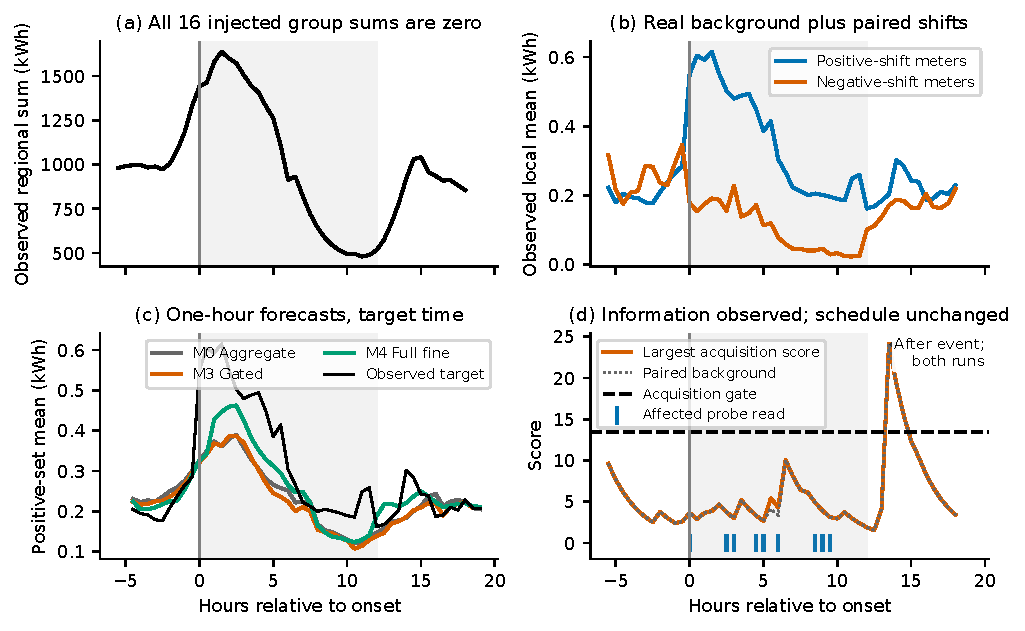
\includegraphics[width=\textwidth]{figures/transparent_episode.pdf}
\caption{Tracing a hidden local change from observations to acquisition. Example b00 uses exact cancellation at nominal magnitude three, selected by first background and fixed family and magnitude before comparison. Gray shading marks the disturbance. (a) Regional demand on observed support varies with the real background, while the injected change sums to zero in every group. (b) Positive and negative meter sets change locally. (c) Forecasts one hour ahead share target times and observed support, without assuming foreknowledge. (d) Affected probes change scores without crossing the acquisition gate during the event. The \DIFaddbeginFL \DIFaddFL{annotated }\DIFaddendFL later \DIFdelbeginFL \DIFdelFL{trigger }\DIFdelendFL \DIFaddbeginFL \DIFaddFL{spike occurs after the disturbance and }\DIFaddendFL also appears on the paired unmodified background. Acquisition remains unchanged and localization is missed. Local sets are evaluator labels unavailable to the policy.}
\label{fig:episode}
\end{figure*}

The example in Figure~\ref{fig:episode} makes the distinction concrete. Group 4 contains 60 affected households. Affected probes appear at onset and on nine event updates, with normalized innovation reaching 3.4411. The maximum acquisition score reaches only 10.0537 against a threshold of 13.4334, while the regional injection remains zero. The traces therefore distinguish information hidden by aggregation from information received without changing acquisition.
\DIFdelbegin \DIFdel{The diagnosis separates measurement access from acquisition responsiveness.
}\DIFdelend 

\DIFdelbegin \DIFdel{The resource comparison quantifies the price of full access. }\DIFdelend Across B, M3 requests 1,123,584 fine records and receives 1,106,434 finite readings\DIFdelbegin \DIFdel{. }\DIFdelend \DIFaddbegin \DIFadd{; }\DIFaddend M4 requests 22,546,944 and receives 22,204,000. \DIFdelbegin \DIFdel{Estimated payloads for fine readings and summaries }\DIFdelend \DIFaddbegin \DIFadd{The request ratio is 20.07. Total estimated consumer payloads }\DIFaddend are 22.52 MB \DIFaddbegin \DIFadd{for M3 }\DIFaddend and 364.95 MB \DIFaddbegin \DIFadd{for M4, each including summaries: fine payloads are 18}\DIFaddend ,\DIFdelbegin \DIFdel{respectively, a factor of 16.2 at the consumer interface}\DIFdelend \DIFaddbegin \DIFadd{665,472 and 361,095,168 bytes, plus 3,854,592 summary bytes per method. All MB are decimal. Fine payload charges 16 bytes per attempted record and 64 per call; M3 makes two calls per update and M4 one. Summaries charge group sums, packed missingness masks and a header. These shared costs reduce the total-payload ratio to 16.21}\DIFaddend . The provider scans all 4,194 meters for each summary, and dense masked arrays generate approximately 5.50 GB of input transfers from host to device per method. Thus the smaller simulated payload establishes an interface tradeoff, without implying reduced measured transfers or provider computation.

\DIFdelbegin \DIFdel{After detail eviction, }\DIFdelend M3 and M4 retain \DIFdelbegin \DIFdel{approximately }\DIFdelend \DIFaddbegin \DIFadd{the same }\DIFaddend 2.365 MB of separator state \DIFdelbegin \DIFdel{per shock update. Conventional retention temporarily requires 41.017 MB. Shared private covariance adds 38.652 MB, and each method's host evidence cache occupies about 0.805 MB. Peak allocation is approximately }\DIFdelend \DIFaddbegin \DIFadd{after eviction. Peak GPU allocation is }\DIFaddend 182.49 MB \DIFdelbegin \DIFdel{on the GPU and 1.73 GB on the host. Each advancing window rebuilds all 16 group messages. Median }\DIFdelend \DIFaddbegin \DIFadd{and median }\DIFaddend complete update time is \DIFdelbegin \DIFdel{around }\DIFdelend \DIFaddbegin \DIFadd{about }\DIFaddend 72 ms, with \DIFdelbegin \DIFdel{similar values across methods. These measurements distinguish retained state, data movement and total update cost, with }\DIFdelend no demonstrated locality or capacity advantage over streaming. \DIFaddbegin \DIFadd{The technical note separates shared covariance, caches, temporary state and host memory.
}\DIFaddend 

\begin{figure*}[!t]
\centering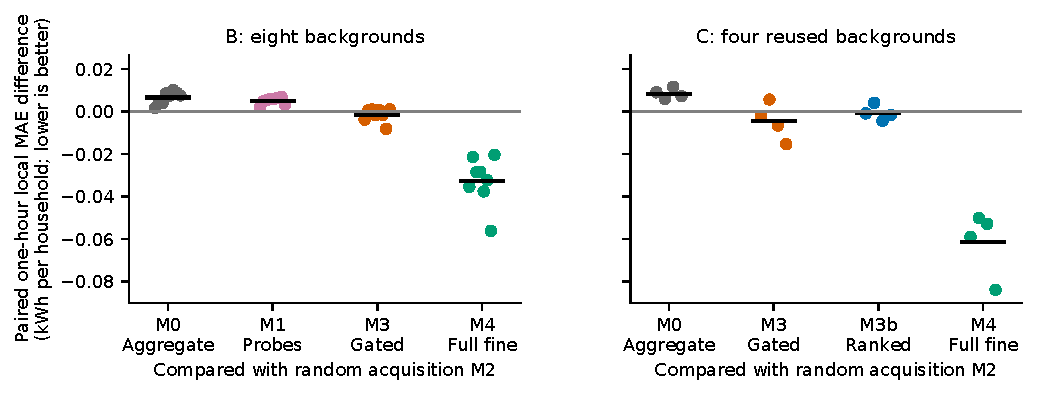
\includegraphics[width=\textwidth]{figures/paired_comparison.pdf}
\caption{Fine access consistently improves local forecasts across backgrounds. Points show paired local MAE differences one hour ahead relative to random acquisition M2. Each dot averages magnitudes and families within one background, and black bars indicate means. Lower is better. B contains eight backgrounds across four weeks. C reuses four backgrounds with fresh seeds and different conditions. M4 receives the larger full access budget. Differences between policies at the restricted budget are small and heterogeneous. The panels describe separate evaluations, with descriptive spread rather than confidence intervals based on independent households.}
\label{fig:paired}
\end{figure*}









\subsection{RQ3. Why responsive scores leave acquisition unchanged}
Most disturbances change acquisition scores without changing which households are read. Reconstruction reproduces all 5,376 original request sequences, finite return counts and active group states, with meter identities and timestamps verified by hashes. The maximum score discrepancy is $1.60\times10^{-14}$. All 96 demand episodes expose an affected fine reading, and 94 expose an affected probe. Innovations change in 96 episodes, group scores in 93, rankings during the event in 86 and the highest ranked group in 17. Yet threshold decisions, active groups and acquisition schedules remain unchanged. No requests are rejected by the budget. Tests with larger innovations successfully change actions when alternatives exist, confirming that the scheduler can respond.

The gate margin explains this behavior. Across all \MarginChecks{} paired updates, the largest score change is smaller than the distance from the background's maximum score to the threshold (Fig.~\ref{fig:path}). Proposition 3 therefore certifies unchanged threshold decisions. Request traces separately confirm unchanged acquisition, accounting for ranking and hold effects. In three episodes, innovation differences disappear when group maxima and score decay are applied. Two episodes without an affected probe still change the reference forecast through macro observations. Checks find no lost disturbance overlay, indexing error or scheduler overwrite.

Alarm calibration presents a separate challenge. M3 alarms on 30/384 unmodified updates, or 7.81\%, against the nominal 2\% target. Both rates concern an alarm on any channel at each update. Applying the same exclusion of eight startup updates gives 17/320, or 5.31\%, compared with 2/88 calibration updates. Startup therefore explains only part of the increase. These are false alarms under the injection protocol, although unmodified backgrounds may contain genuine unlabeled changes.

In corrective panel C, M3b changes schedules in three of 12 demand episodes. M3b, M3 and random acquisition each correctly localize two. Local MAE is 0.2660 kWh for M3b, compared with 0.2621 for M3, 0.2667 for random and 0.2053 for streamed fine inference. M3b's 0.25\% average improvement over random varies across backgrounds and does not establish an acquisition advantage. M3 remains better on the primary average. Control alarm rates are 14/192, or 7.29\%, for M3b and 15/192, or 7.81\%, for M3, both above target. Restricted budget methods use 209 attempts per update and an estimated 2.666 MB of fine payload across C, with small differences in finite returns. \DIFdelbegin \DIFdel{These comparisons distinguish making acquisition responsive from making it useful}\DIFdelend \DIFaddbegin \DIFadd{This small, reused-background panel does not establish superiority or equivalence}\DIFaddend .



\begin{figure*}[!t]
\centering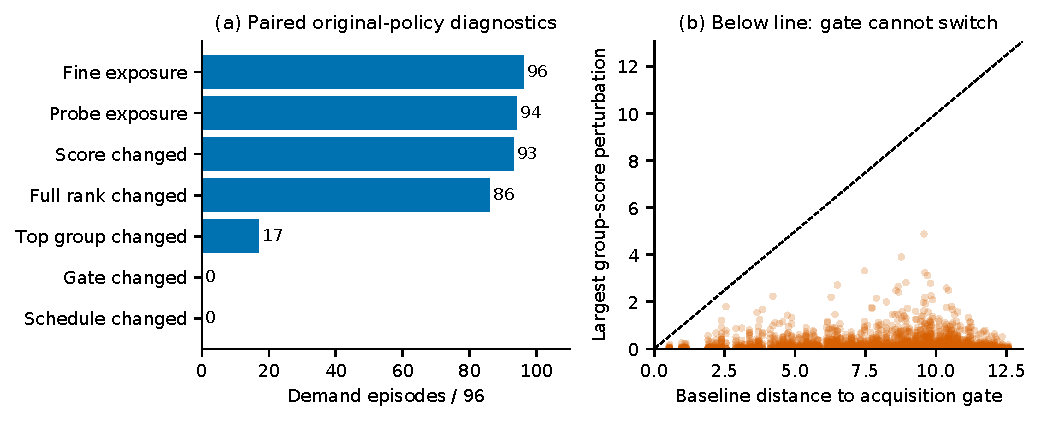
\includegraphics[width=\textwidth]{figures/acquisition_path.pdf}
\caption{Locating the gap between changed observations and unchanged acquisition in panel B. (a) Counts cover 96 demand episodes. Rankings are compared during disturbances, while score comparisons cover the replay. The conditions are distinct and do not form a strict funnel. (b) Score changes are compared with the background's distance to the acquisition threshold. All 4,608 paired updates satisfy the sufficient condition for unchanged gate decisions, including zero changes omitted from the scatter. Meter identities and timestamps independently verify that request sequences remain unchanged.}
\label{fig:path}
\end{figure*}







\subsubsection{Identifying timing and calibration requirements}
Corrective traces identify where acquisition can be improved. In the changed exact cancellation and localized episodes, selection first changes at lags eight and nine, adding 120 and 77 requests for affected meters. Both occur after the \DIFdelbegin \DIFdel{detection window at lags zero through six}\DIFdelend \DIFaddbegin \DIFadd{original scoring window and the extended lag-0--6 window used by the timing diagnostic}\DIFaddend . The third schedule changes at lag six but adds no affected meter. Thus the correction reaches additional affected meters only after the scoring deadline. A separate audit checks missingness and actual perturbations to distinguish affected identities from informative returned readings.

Alarm calibration provides the second explanation. Across fresh demand episodes, acquired fine innovations within \DIFdelbegin \DIFdel{the window }\DIFdelend \DIFaddbegin \DIFadd{lags 0--6 }\DIFaddend reach at most 15.85, below M3b's threshold of 20.586, compared with 19.708 for M3. Its two correct group localizations therefore come through the macro channel. These results identify timely targeting and alarm calibration as distinct design priorities. Evaluating alternatives requires sequential replay because changed acquisitions alter subsequent evidence.

Fixed and adaptive representations agree under identical evidence in all 5,376 original and 960 corrective or diagnostic updates. This consistency isolates additional observations as the source of forecast improvement.
\DIFdelbegin \DIFdel{Together, the comparisons provide a practical diagnosis of how information access, acquisition timing and alarm decisions contribute to useful refinement.
}\DIFdelend 














\section{Discussion}
The \DIFdelbegin \DIFdel{study provides a practical methodology for determining where additional detail creates value in a regional energy twin. Its contribution combines controlled comparisons, mathematical consistency checks and traces of actual acquisition decisions. Together, these establish which predictions survive changes in representation, what additional observations contribute and how decision rules affect the use of that information. This gives designers a clearer basis for choosing where to invest in storage, measurement access and acquisition logic.
}%DIFDELCMD < 

%DIFDELCMD < %%%
\DIFdel{The results demonstrate that consistent movement between regional and household views is achievable within one probabilistic model. New observations update predictions across groups through the shared state, including households whose fine readings remain unavailable. This is a useful capability for consumers that receive regional summaries but can request only selected local measurements. The comparison with streamed inference also identifies the appropriate resource baseline. Memory savings should be assessed alongside restoration, shared storage and data movement, rather than interpreted automatically as increased capacity.
}%DIFDELCMD < 

%DIFDELCMD < %%%
\DIFdel{The acquisition diagnosis adds a complementary design lesson. Information can reach a consumer and change its scores without changing its requests. In the tested policy, the acquisition gate suppresses this response even though the observation budget is still spent. The correction then separates responsiveness from timeliness by showing that additional requests for affected meters arrive after the detection deadline. These findings make allocation, timing and alarming independently testable parts of the system. They provide specific mechanisms to examine when increasing detail fails to improve a consumer's decisions. }%DIFDELCMD < 

%DIFDELCMD < %%%
\DIFdel{For data sharing, the practical implication is that an interface should describe both available queries and the evidence supporting them. Useful records include }\DIFdelend \DIFaddbegin \DIFadd{results support a diagnostic methodology, not an operationally validated acquisition system. Table~\ref{tab:guidance} distinguishes checks supported by this study from remedies that require new validation. Information-sharing interfaces should record }\DIFaddend which measurements were acquired, when they entered inference and how they influenced \DIFdelbegin \DIFdel{subsequent requests.
The study shows how these records support reproducible comparisons and prevent forecast gains from being attributed to representation changes alone.
}\DIFdelend \DIFaddbegin \DIFadd{requests.
}\DIFaddend 



\DIFdelbegin %DIFDELCMD < 
%DIFDELCMD < %%%
\DIFdelend Predictive reliability also requires calibration beyond numerical agreement. \DIFdelbegin \DIFdel{In panel B's unmodified controls, M3}\DIFdelend \DIFaddbegin \DIFadd{Panel A}\DIFaddend 's nominal 90\% regional \DIFdelbegin \DIFdel{intervals cover 72.14\%of observations. Calibration adjustment raises coverage }\DIFdelend \DIFaddbegin \DIFadd{coverage is only 59.4\%. For M3's one-hour regional intervals on B's unmodified controls, coverage is 72.14\%, rising }\DIFaddend to 84.12\% \DIFdelbegin \DIFdel{, indicating progress while remaining below the target. This provides a clear distinction between consistent computation and reliable uncertainty estimates}\DIFdelend \DIFaddbegin \DIFadd{after adjustment. Alarm calibration is separate and uses only 88 post-startup updates; its realized rates also exceed the 2\% target. Neither numerical agreement nor the retrospective threshold sweep establishes reliable calibration}\DIFaddend .

The findings concern retrospective replay over four development weeks, \DIFdelbegin \DIFdel{using }\DIFdelend synthetic disturbances and simulated \DIFdelbegin \DIFdel{provider groups within a sampled household population. Fresh seeds reuse existing backgrounds and therefore do not provide independent validation on unseen periods. The archive establishes substantial ingestion scale, while the 384 dimensional common separator represents a smaller inference task. Dense transfers and reconstruction at each window shift remain opportunities for implementation improvement, with no demonstrated capacity advantage over streaming}\DIFdelend \DIFaddbegin \DIFadd{providers in a sampled population. Synthetic index-based groups do not establish performance for geographical or feeder groups. Window restarts discard earlier evidence; their forecast and uncertainty effects are unmeasured. Panel C has only 12 demand episodes and reuses B's backgrounds, so fresh seeds are not independent chronological validation. The 384-dimensional separator is a modest inference problem: processing 167.93 million archive rows does not demonstrate comparable inference scalability}\DIFaddend .

\DIFdelbegin \DIFdel{The next study can build directly on this diagnosis by testing whether earlier group ranking delivers informative readings before a fixed deadline while maintaining the intended alarm rate on separate chronological backgrounds. Such sequential evaluation would connect the demonstrated value of fine observations to the practical design of more effective acquisition policies}\DIFdelend \DIFaddbegin \DIFadd{Independent chronological validation is needed before operational use. April--December 2013 remains sealed and is a natural future evaluation period, not new validation in this revision. Earlier ranking would require sequential testing because changed requests alter later evidence}\DIFaddend .


\DIFaddbegin 
\DIFaddend \section{Conclusion}
This study provides a reproducible methodology for evaluating how local detail contributes to a regional energy twin. Controlled comparisons demonstrate consistent refinement between regional and household views and identify additional observations as the source of improved local forecasts. Comparison with streamed inference places the measured storage savings against a realistic capacity baseline.

Execution traces make the connection between information and decisions explicit. Disturbances change acquisition scores, but the gate prevents those changes from affecting requests. The targeted correction reveals a further timing constraint, with additional requests for affected meters arriving after the detection deadline. These findings identify concrete design priorities without establishing a superior acquisition policy.

\DIFdelbegin \DIFdel{The contribution is a linked evaluation of representation, observation access and decision behavior. It }\DIFdelend \DIFaddbegin \DIFadd{This diagnostic evaluation }\DIFaddend gives twin designers \DIFdelbegin \DIFdel{practical }\DIFdelend controls for assessing memory tradeoffs, measuring \DIFdelbegin \DIFdel{the value of fine observations }\DIFdelend \DIFaddbegin \DIFadd{information value }\DIFaddend and locating barriers to timely action\DIFdelbegin \DIFdel{. This connects the detail a regional twin retains with the information it gains and the decisions that information can support}\DIFdelend \DIFaddbegin \DIFadd{, without claiming demonstrated operational performance}\DIFaddend .





\bibliographystyle{IEEEtran}
\bibliography{references}
\end{document}
